\chapter{Android Studio}

\section{Installation}
Android studio er gratis og kan installeres på Windows, Mac og Linux.\\
Man kan google Android Studio eller følge dette link:\\
\url{https://developer.android.com/studio/index.html}

På deres hjemmeside har de guides og videoer, som kan hjælpe dig.
Først downloader du Android Studio og åbner derefter den hentede fil.

\section{Oprettelse af projekter}
Efter du har installeret Android Studio, åbner du det, og hvis du ikke har et projekt åbent kommer du til velkomst-menuen. Der trykker du "new project".

Så skal du skrive, hvad din app skal hedde, dit domæne (ikke så vigtigt, hvis du ikke vil sælge den) og hvor appen skal ligge på din computer. I \autoref{fig:createproject} har jeg valgt Min Clicker app, og valgt at den skal ligge i mappen Clickerapp. 
\begin{figure}[h]
	\marginnote{\qrcode{https://raw.githubusercontent.com/UNFDanmark/SDC-Faglig-Bog/master/sections/ekstra/studio/figures/CreateProject.png}}
	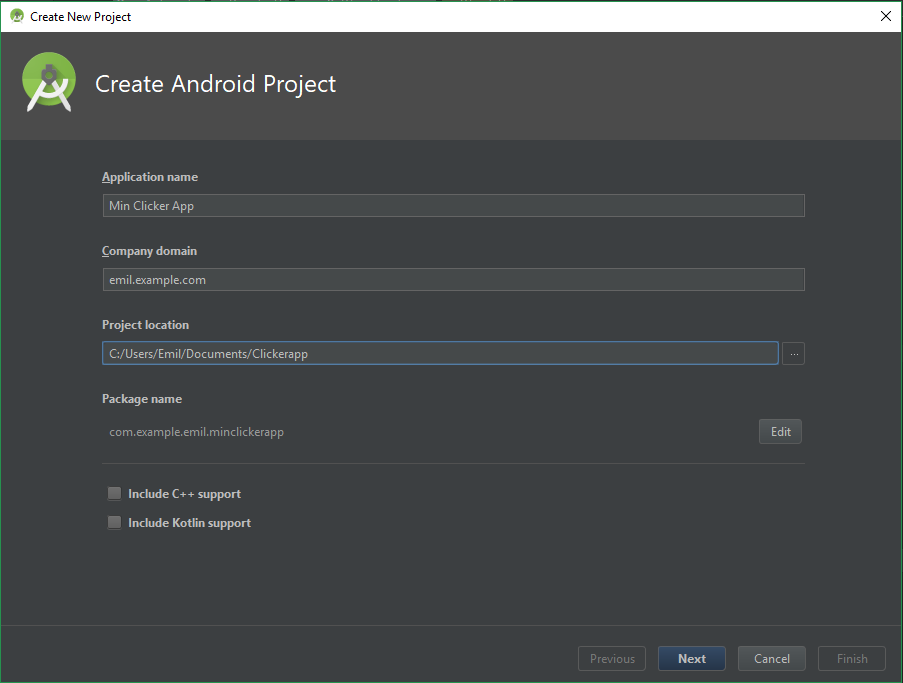
\includegraphics[width=\textwidth]{CreateProject}
	\caption{Opret Android projekt}
	\label{fig:createproject}
\end{figure}
Det er godt at lave en mappe til sit projekt, så man let kan finde det igen. 

Bagefter skal man vælge hvad for en version af Android, den laveste version skal kunne installeres på. Se \autoref{fig:API}. Man kan også lave til andre platforme, men det vil jeg ikke komme længere ind på. 
\begin{figure}[h]
	\marginnote{\qrcode{https://raw.githubusercontent.com/UNFDanmark/SDC-Faglig-Bog/master/sections/ekstra/studio/figures/API.PNG}}
	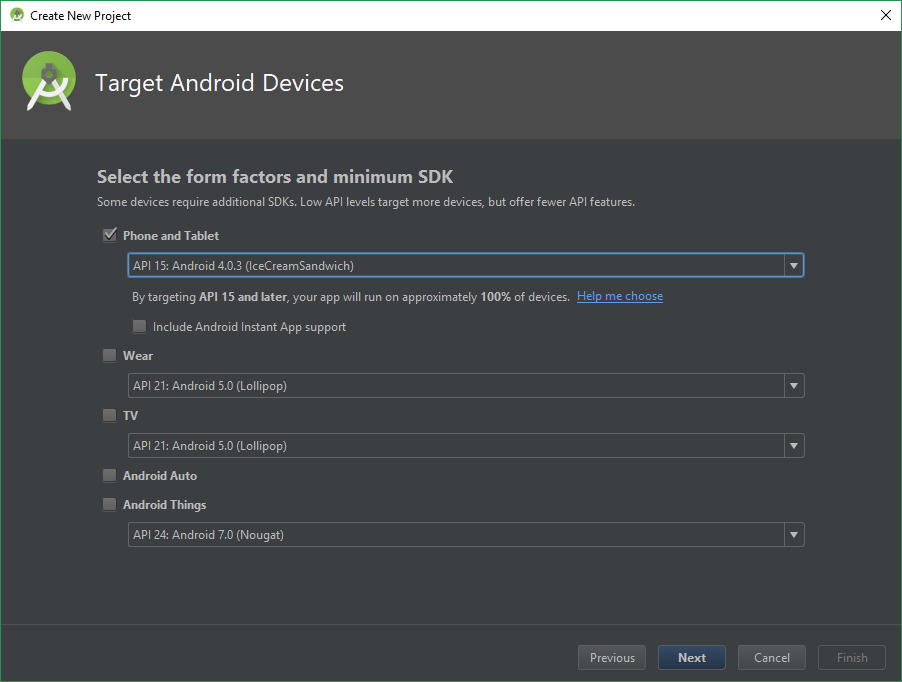
\includegraphics[width=\textwidth]{API}
	\caption{Android version}
	\label{fig:API}
\end{figure}

Derefter vælger man en Activity.
Man kan vælge en pre-defineret Activity med noget funktionalitet, eller bare tage en hel tom Activity som jeg har gjort i \autoref{fig:Activiy}.

\begin{figure}[h]
	\marginnote{\qrcode{https://raw.githubusercontent.com/UNFDanmark/SDC-Faglig-Bog/master/sections/ekstra/studio/figures/Activity.PNG}}
	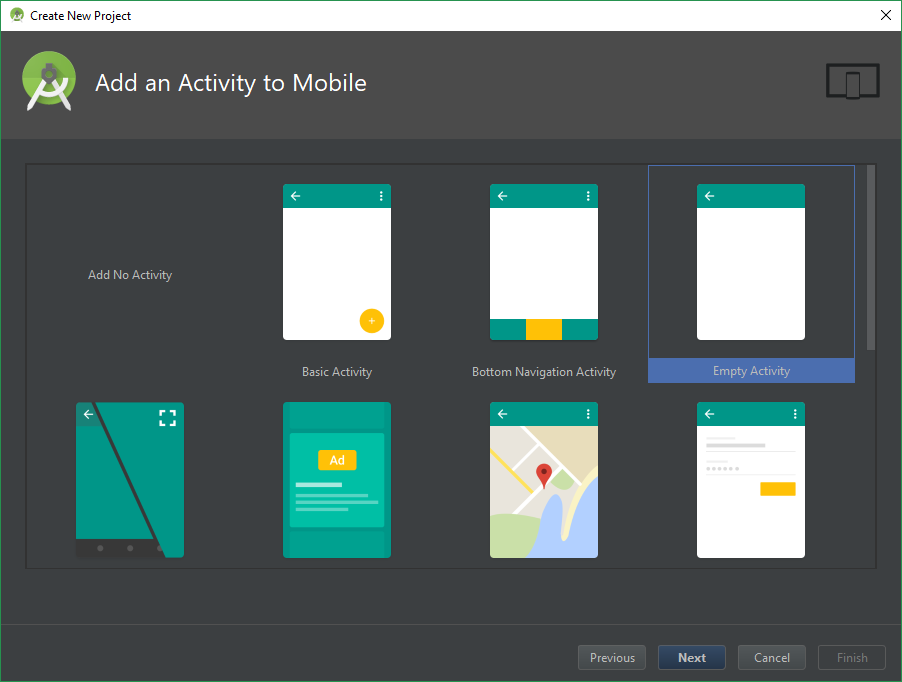
\includegraphics[width=\textwidth]{Activity}
	\caption{Oprettelse af activity}
	\label{fig:Activiy}
\end{figure}

Så skal du navngive din activity, hvis det er din hoved activity, så skal du kalde den MainActivity, som jeg gør i \autoref{fig:Config Activiy} 

\begin{figure}[h]
	\marginnote{\qrcode{https://raw.githubusercontent.com/UNFDanmark/SDC-Faglig-Bog/master/sections/ekstra/studio/figures/ConfigActivity.PNG}}
	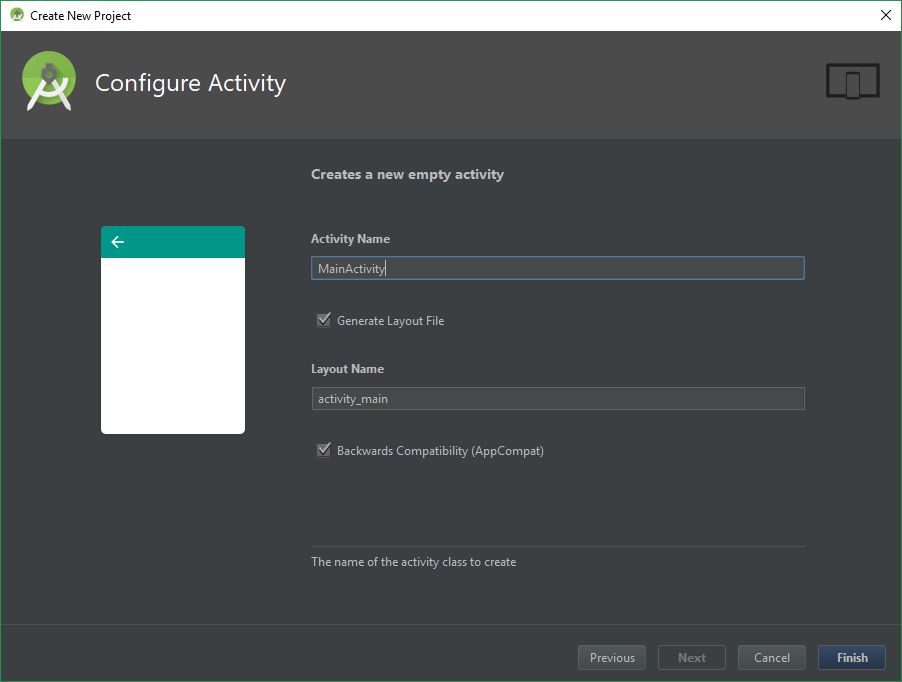
\includegraphics[width=\textwidth]{ConfigActivity}
	\caption{Navngivning af activity}
	\label{fig:Config Activiy}
\end{figure}

Nu vil Android Studio så sætte basis tingene op.

\FloatBarrier

\section{Eksempel på en meget simpel app}

Nu da vi har fået lavet skelettet til appen, skal vi have knapper og text felter.

\begin{figure}[h]
	\marginnote{\qrcode{https://raw.githubusercontent.com/UNFDanmark/SDC-Faglig-Bog/master/sections/ekstra/studio/figures/App.PNG}}
	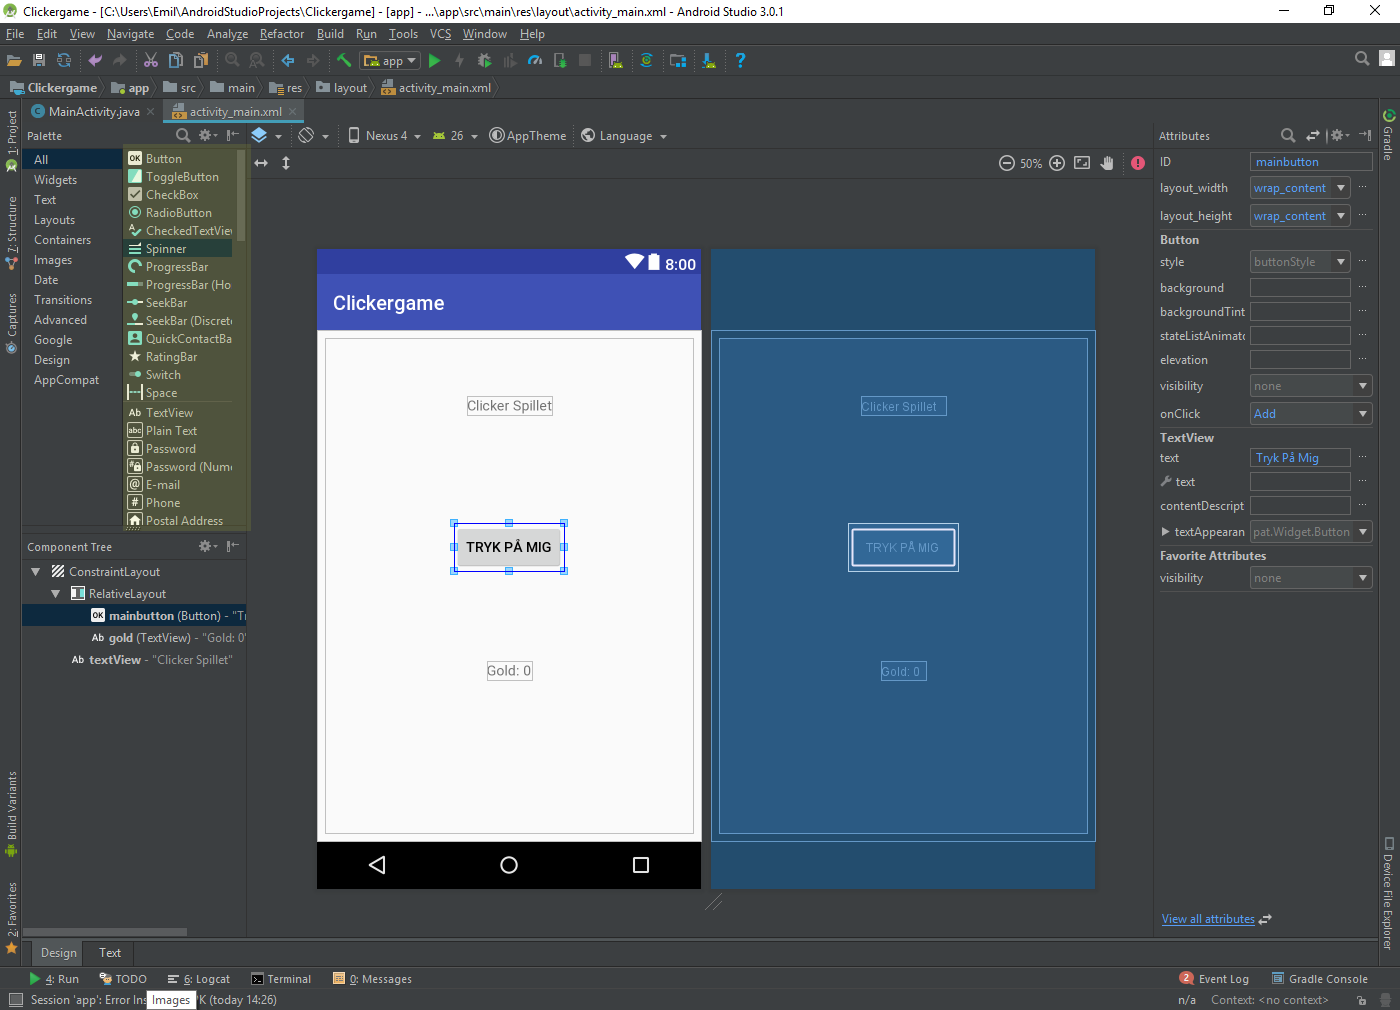
\includegraphics[width=\textwidth]{App}
	\caption{Knapper og tekstfelter}
	\label{fig:App}
\end{figure}

De findes i paletten som er markeret med gul i \autoref{fig:App}. 

"Tryk på Mig" firkanten er en Button, og "Gold: 0" er et Textview. 
Knapperne og tekst felterne kan ses i component tree i venstre hjørne, og der kan du også se, hvis du har andre komponenter.

Hvis du har en knap eller et tekstfelt markeret, kan du se dets attributes i højre side.

Det er vigtigt, at hver knap eller tekst felt har et ID, så de kan findes i koden. Ellers kan du bare rode rundt med de andre. 

Der skulle også være lavet en MainActivity java fil.

I \autoref{lst:Java} kan du se, hvad jeg har skrevet i min MainActivity. 

\begin{JavaCode}{Eksempel på MainActivity}{lst:Java}
	public class MainActivity extends AppCompatActivity {
		int gold = 0;
		
		Button button;
		TextView textView;
		
		@Override
		protected void onCreate(Bundle savedInstanceState) {
			super.onCreate(savedInstanceState);
			setContentView(R.layout.activity_main);
			
			button = (Button) findViewById(R.id.mainbutton);
			textView = (TextView) findViewById(R.id.gold);
			
			button.setOnClickListener(new View.OnClickListener() {
				@Override
				public void onClick(View view) {
					gold++;
					textView.setText("Gold: " + gold);	
				}
			});
		}
	}
\end{JavaCode}

Jeg har sat en variabel gold, som har styr på guld beholdningen. 

Derefter har jeg lavet de to variabler, Knap og tekst. 

På oncreate, som er når appen starter, har jeg sat den til at finde Knappen og tekst feltet, som jeg satte ind. 

Derefter har man brug for en onclicklistener, som opfanger når folk trykker på knappen. 

Så det, der sker når folk trykker på knappen, er at gold øges med 1 og tekst feltet ændres til Gold og derefter, hvor meget huld man har. 

Tilsidst kan appen afprøves på en android mobil eller på en emulator. På mobilen er man nødt til,   at slå filoverførsel til. 






